%---
\section{Introduction}\label{sec:intro}\label{sec:introduction}

\dsf\ is a Liquid Argon Time Projection Chamber (\lar\ \tpc), operated in the Gran Sasso National Laboratory (LNGS) in Italy to search for nuclear recoils induced by weakly interacting massive particles (WIMPs). A first physics result was reported in \cite{ds:ds-50:firstpaper} based on 50 live days of data collected with Atmospheric Argon (AAr), providing the most sensitive limit on a dark matter search using a \lar\ \tpc\ to date with a 90\% CL upper limit on the WIMP-nucleon spin-independent cross section of $6.1 x 10^{-44}$ cm$^2$ for a WIMP mass of 100 GeV/c$^2$.  %along with two other key results: ar bg can be suppressed for ton-scale experiments using \uar and efficiency of the veto 

The \dsf\ apparatus has been described in detail in \cite{ds:ds-50:firstpaper}, but for the reader's convenience a short reminder is given. As shown in fig.~\ref{fig:wholeAssembly_insideDetectors} it features a \lar\ \tpc\ surrounded by a 30 t liquid scintillator-based veto (LSV) system, which in turn is housed in a water Cerenkov detector (\wcd), both of which help to measure in-situ and suppress radiogenic and cosmogenic backgrounds. On top of the \wcd\ there is a radon-free clean room (CRH) which houses the cryogenic supply system, the electronics and slow control software, among other things (Fig.~\ref{fig:CALIS_photos}). The inside of the \lsv\ is accessible from CRH through four access ports nick named organ pipes, which end at their top in gate valves. 

%After this introduction the CALIS design requirements and hardware realization are described in Sec.~\ref{sec:hardware}. Calibration campaigns and some of their physics highlights are discussed in Sec.~\ref{sec:CalibCampaigns}, before concluding in Sec.~\ref{sec:Conclusion}.

\begin{figure}[htbp]
 \centering
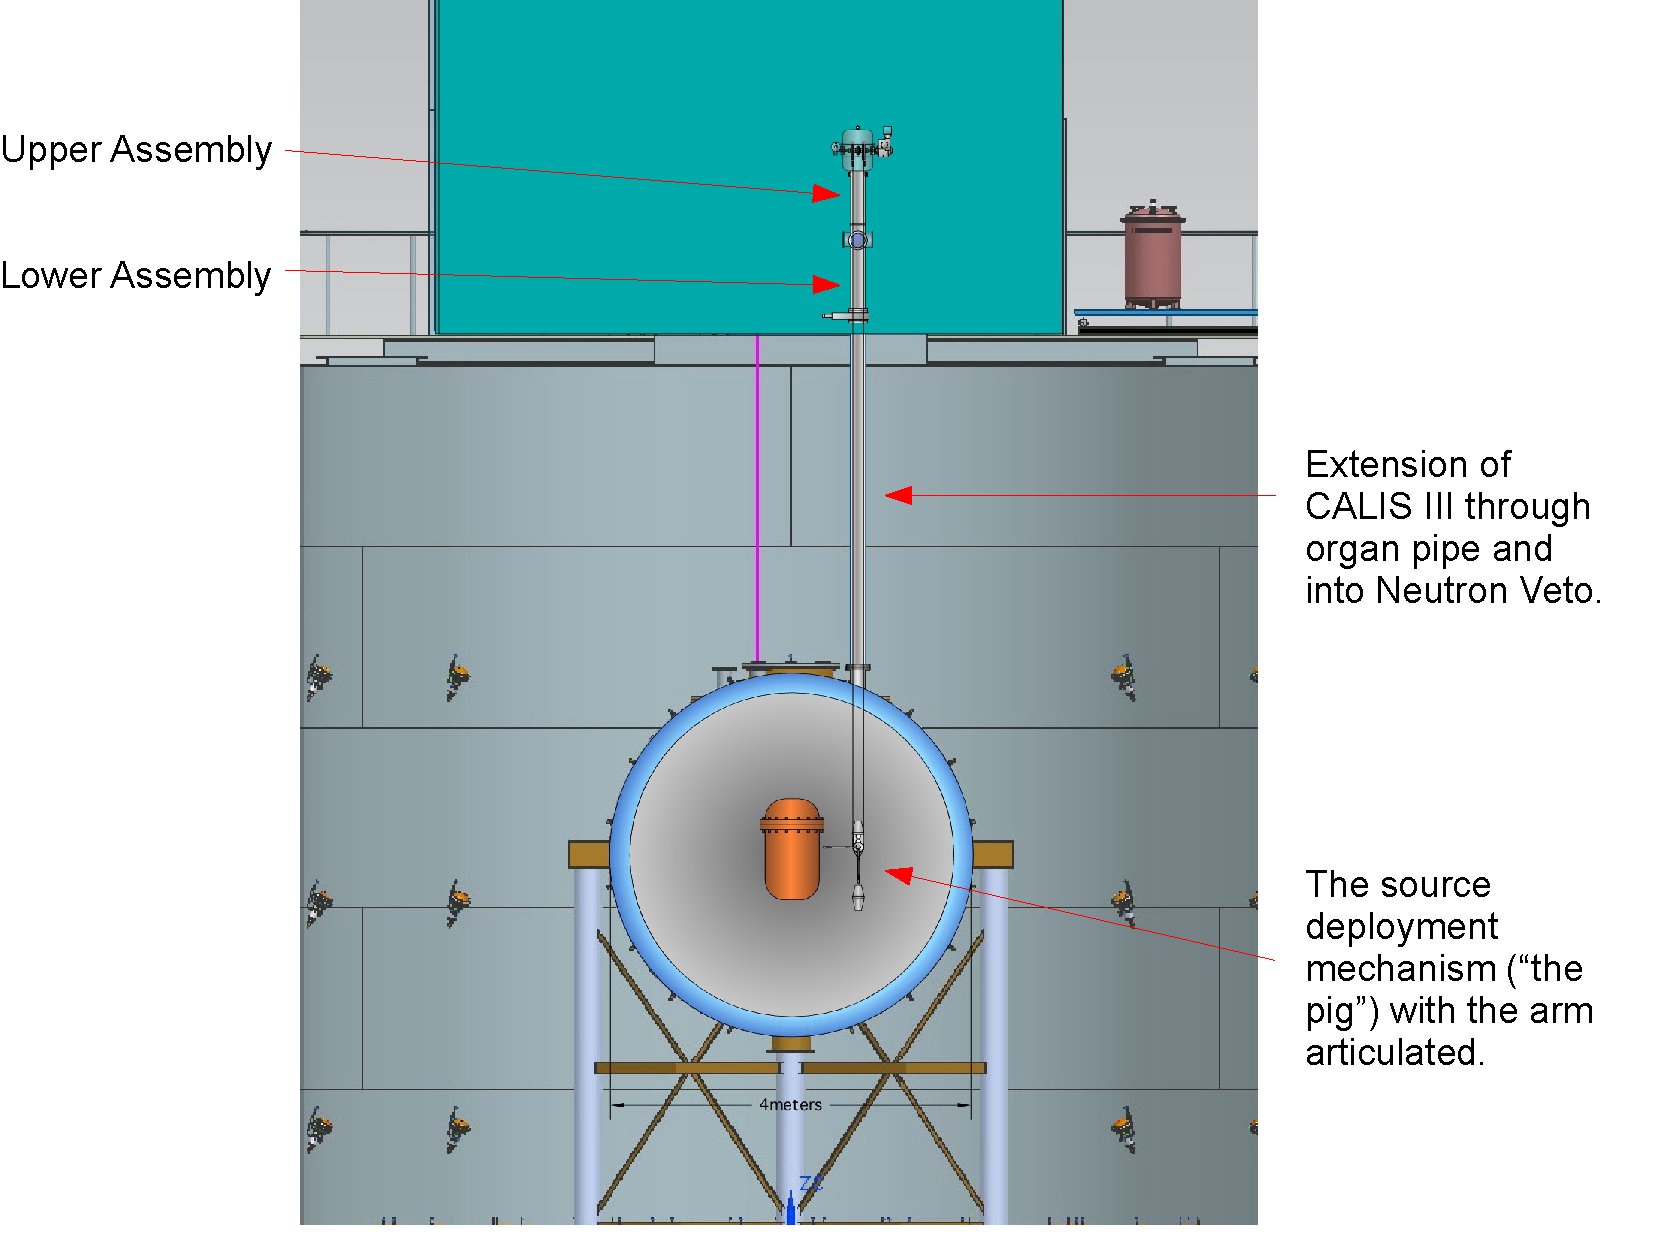
\includegraphics[width=\textwidth]{Figures/wholeAssembly_insideDetectors}
\caption{A conceptual drawing of CALIS installed in the radon-suppressed clean room CRH atop the water Cerenkov detector (WCD) and with the deployment device containing the source  %%% not introduced yet
deployed in the liquid scintillator veto (LSV) next to the liquid argon time projection chamber's (\lar\ \tpc) cryostat. The clean room and the LSV are connected through four %%%how long?
access ports nick named organ pipes (only one of which is drawn in the sketch above: (1)). All four organ pipes end in CRH at gate valves (2) which can be manually opened or closed. During normal operations all four organ pipes are closed. Not included in the sketch are tubes connecting the cryogenic systems in CRH to the cryostat in the LSV ((3) and (4)).\label{fig:wholeAssembly_insideDetectors}}
\end{figure}

\begin{figure}[htbp]
 \centering
\subfigure{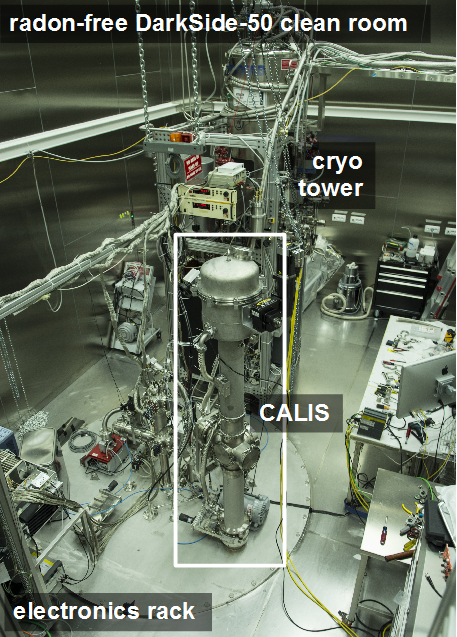
\includegraphics[width=0.335\textwidth]{./Figures/CALISinCRH.png}}
\subfigure{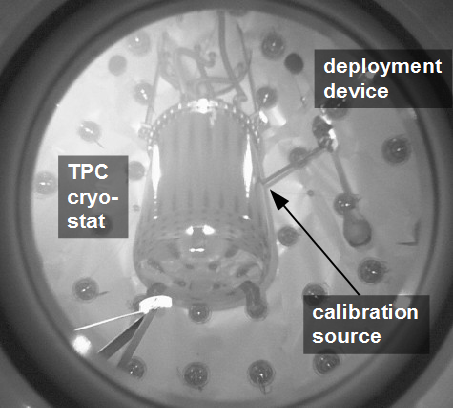
\includegraphics[width=0.52\textwidth]{./Figures/Next2Cryostat.png}}
\caption{\textit{left}: CALIS after installation inside the CRH room. The organ pipe is 80 cm off-center with respect to the TPC center in the horizontal XY plane. \textit{right}: Photograph taken with a camera looking upwards into the LSV from the bottom. It shows the source deployment device deployed through one of the organ pipes visible on the top right. The arm is articulated and the source is next to the cryostat of the \lar\ \tpc.
\label{fig:CALIS_photos}}
\end{figure}



%time line plot, how did the veto change during the calibration campaigns - allowing for systematics studies.
%table on what was the goal of each campaign. What sources were used


%safety requirements

%design section
%installation: before, after

%how sources were selected? DAQ constraints, avoid pile-up, maximize time used for calibration
